\documentclass{standalone}
\usepackage{amstext}
\usepackage{tikz}
\usetikzlibrary{shapes,arrows,fit}
\begin{document}
\providecommand{\mylabel}[1]{\begin{minipage}{2cm}\begin{center}#1\end{center}\end{minipage}}
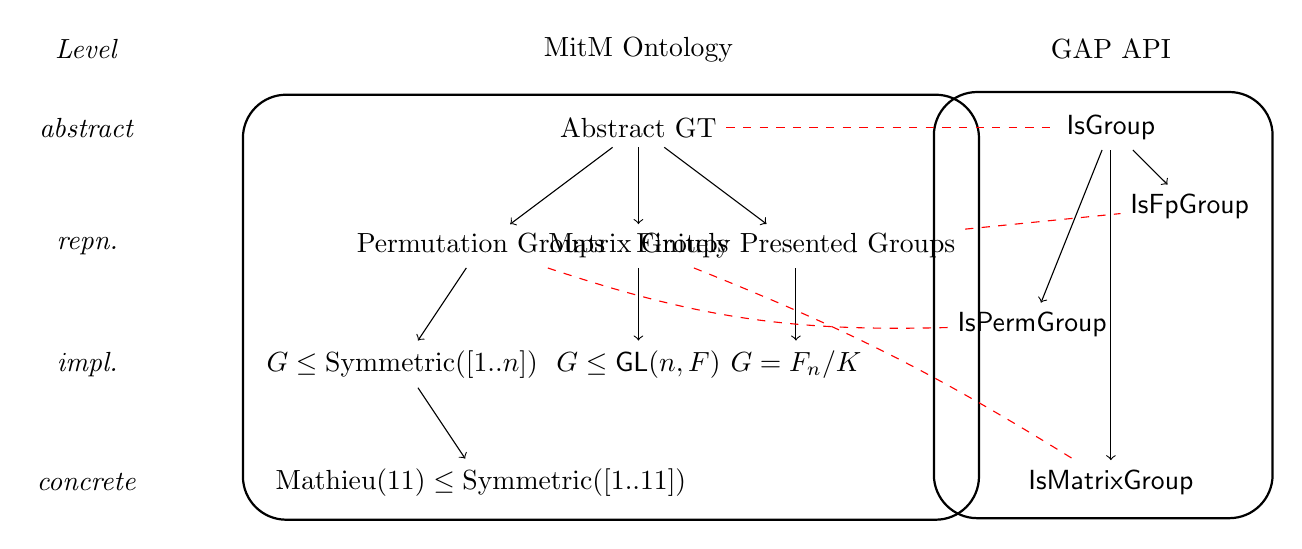
\begin{tikzpicture}
\node (mitm) at (-4,8.5) {\emph{Level}}; 
\node (a) at (-4,7.5) {\emph{abstract}}; 
\node (b) at (-4,6) {\emph{repn.}}; 
\node (c) at (-4,4.5) {\emph{impl.}}; 
\node (d) at (-4,3) {\emph{concrete}}; 

\node (mitm) at (3,8.5) {MitM Ontology};

\node (grouptheory) at (3,7.5) {Abstract GT};
\node (permgrp) at (1,6) {\mylabel{Permutation Groups}};
\node (matgrp) at (3,6) {\mylabel{Matrix Groups}};
\node (finpresgrp) at (5,6) {\mylabel{Finitely Presented Groups}};
\draw[->] (grouptheory) -- (permgrp);
\draw[->] (grouptheory) -- (matgrp);
\draw[->] (grouptheory) -- (finpresgrp);

\node (symm) at (0,4.5) {$G\leq\text{Symmetric}([1..n])$};
\node (glnf) at (3,4.5) {$G\leq\textsf{GL}(n,F)$};
\node (fnk) at (5,4.5) {$G=F_n/K$};
\draw[->] (permgrp) -- (symm);
\draw[->] (matgrp) -- (glnf);
\draw[->] (finpresgrp) -- (fnk);

\node (mathieu) at (1,3) {$\text{Mathieu}(11)\leq\text{Symmetric}([1..11])$};
\draw[->] (symm) -- (mathieu);

 \node[draw,thick,fit=(grouptheory) (permgrp) (matgrp) (finpresgrp) (symm) (glnf) (fnk) (mathieu),
                   rounded corners=.55cm, inner sep=5pt] (mitmcloud) {};
                   
\node (gap) at (9,8.5) {GAP API};

\node (isgrp) at (9,7.5) {\textsf{IsGroup}};

\node (ispermgrp) at (8,5) {\textsf{IsPermGroup}};
\node (ismatgrp) at (9,3) {\textsf{IsMatrixGroup}};
\node (isfpgrp) at (10,6.5) {\textsf{IsFpGroup}};
\draw[->] (isgrp) -- (ispermgrp);
\draw[->] (isgrp) -- (ismatgrp);
\draw[->] (isgrp) -- (isfpgrp);

 \node[draw,thick,fit=(isgrp) (ispermgrp) (ismatgrp) (isfpgrp),
                   rounded corners=.55cm, inner sep=5pt] (gapcloud) {};
                   
\draw[red,dashed] (grouptheory) -- (isgrp);
\draw[red,dashed] (permgrp) to[bend right=10] (ispermgrp);
\draw[red,dashed] (matgrp) to[bend left=5] (ismatgrp);
\draw[red,dashed] (finpresgrp) -- (isfpgrp);

%
%\node (Int) at (6,8.5) {Interfaces};
%
%\node (TT) at (4.9,3.5) {Type Theory};
%\node (ST) at (7.6,4.2) {Set Theory};
%\draw[<->,dotted] (TT) -- (ST);
%
%\node (Reals) at (4.7,4.8) {\textsf{Numbers}};
%\node (Nat) at (4.7,6) {$\mathbb N$};
%\draw[\arrowtipmono-\arrowtip] (Reals) -- (Nat);
%
%\node (FOrd) at (7.2,5.5) {Finite Ordinals};
%
%\node (PA) at (6,7) {Peano Axioms};
%\draw[<-] (FOrd) -- (PA);
%\draw[<-] (Nat) -- (PA);
%\draw[\arrowtipmono-\arrowtip] (ST) -- (FOrd);
%
% \node[draw,thick,fit=(ST) (Reals) (Nat) (FOrd) (PA) (TT),
%                   rounded corners=.55cm, inner sep=10pt] (PVScloud) {};
%
%\node (gap) at (11,8.5) {GAP API};
%
%\node (MNat) at (11,7) {\textsf{Nat}};
%\node (MOrd) at (11,3) {\textsf{Ordinals}};
%\draw[\arrowtipmono-\arrowtip] (MOrd) -- (MNat);
%
% \node[draw,thick,fit=(MNat) (MOrd),
%                   rounded corners=.55cm, inner sep=5pt] (PVScloud) {};
%
%\draw[red] (PVSfnd) -- (TT);
%\draw[red] (Mizfnd) -- (ST);
%\draw[red] (MOrd) -- (ST);
%\draw[red] (PVNat) -- (Nat);
%\draw[red] (PVnf) -- (Reals);
%\draw[red] (MNat) -- (FOrd);
%
%\draw[<->,dotted] (TT) -- (Reals);
%\draw[<->,dotted] (ST) -- (Reals);

\end{tikzpicture}
\end{document}

%%% Local Variables:
%%% mode: latex
%%% TeX-master: t
%%% End:
